\documentclass[a4paper]{article}
\usepackage{amsmath}
\usepackage{subfigure}
\usepackage{graphicx}
\usepackage{geometry}
\usepackage{floatrow}
\usepackage{layout}
\usepackage{amssymb} 
\usepackage{multirow}
\usepackage{caption}
\geometry{margin=1in}
\usepackage{authblk}
 \usepackage{indentfirst}
\begin{document}
\title{\textbf{\huge{Optical fiber technology and its applications}}}
\author{\textbf\large{Luo Bowen}}
%\affiliation{The	College,	University	of	Chicago,	Chicago,	Illinois	60637,	USA}
\affil{\textbf{Sichuan University,	Chengdu,		China}}
\date{\today}
%	Abstract
\maketitle
\begin{abstract}
Optical fibers use the principle that light travels through fine glass fibers by total reflection. In 1870, John Tyndall made the first use of total internal reflection to transmit light. In front of an audience at the royal society of art in London, he conducted an experiment in which light from the surface of a bucket of water could be transmitted through a small hole in the side of the bucket. He cut a small hole in the side of a large barrel and filled it with water. Shining a strong light on the water in the bucket, he turned off the light in the room, and saw that the light coming into the water flowed out with the water from the holes, and fell to the surface with the curved water, creating a light beam on the ground. Tyndall's discovery inspired scientists to use very fine filaments of glass, called fibre-optic fibres, as "wires" for light, and since then amazing progress has been made. Today's fiberglass has become a viable means of optical transmission in optical communications. Today, I will introduce to you this advanced science, the principle and application of optical fiber.Optical fiber communication has many advantages, such as large transmission capacity, small loss, light weight, good confidentiality and so on. If communication is like a road, then the wider the frequency band of the communication line, the more information it is allowed to transmit, and the larger the information capacity. Optical fiber has many applications in many fields, such as communication, computer LAN, and power system monitoring. With the progress of the society and the increasing demand for information, the transmission capacity of digital system is constantly increasing, and people urgently need to establish a unified worldwide communication network. In this situation, many shortcomings of the existing PDH are gradually exposed, mainly in North America, Western Europe and Asia, the three digital systems are not compatible with each other, there is no unified standard optical interface in the world, making the establishment of international telecommunications network and operation, management and maintenance are very complex and difficult.Optical fiber communication has many advantages, such as large transmission capacity, small loss, light weight, good confidentiality and so on.When the Angle of the incident light reaches or exceeds a certain Angle, the refracted light will disappear and all the incident light will be reflected back, which is the total reflection of light. Different substances have different refractive angles to light of the same wavelength, that is, different substances have different refractive indexes, and the same substances have different refractive angles to light of different wavelength. Fiber optic communication is based on the above principles.
\end{abstract}\maketitle
%	\tableofcontents
%%	Main	body	starts	here
%	Description	of	Section	1
\section{introduction}
\label{sec:Intro}
%	Introduction
%	What is	the	background	and	the	context?
Light is an electromagnetic wave visible to the naked eye. In science, light is sometimes defined as all electromagnetic waves. Light consists of an elementary particle called a photon. It has the characteristics of particle and wave, or wave-particle duality. Optical fiber propagates through optical fiber through total reflection, which is a special situation of reflection. Light has both reflection and refraction phenomena. The reflection of light is like this: the light is blocked in a plane and the incident Angle and reflection Angle are the same. The refraction of light is the deflection of light as it passes through a medium of different densities. The energy loss of light in the refraction process is much greater than that of light in the reflection process. Light can transmit both information and energy, which is a very advanced and feasible technology in today's society. However, how to convey the information and the quality of the information is a more meaningful question. So, people invented optical fibers to transmit light, and we can read information from light. I will do an experiment to test the quality of the information that I come up with. In the experiment, we can see that the optical fiber clearly propagates the video information. We show here the quality of the information transmitted using optical fiber. It can be seen that the information transmitted by optical fiber is very reliable, free from interference, and of great practical value. So we can use fiber optics to transmit information somewhere else, to connect to the Internet. We hope that in the experiment, we can see the image on the display and the image we see on the camera as accurately as possible, and receive electromagnetic radiation from the surrounding wires, and also present a stable image. When the optical fiber moves, we also hope that the image displayed on the display can be stable output, we can see the clear image.
\\

Optical fiber is widely used in communication, computer LAN, power system monitoring and other fields. With the progress of the society and the information demand growing, increasing number system of transmission capacity, there is an urgent need to build a unified global communications network. In this case, many existing PDH gradually exposed shortcomings, mainly concentrated in North America, Western Europe and Asia three digital system is not compatible with each other, there is no unified standard optical interface, make the establishment and operation of international telecommunication network, is a very complex and difficult to manage and maintain. Optical fiber communication has a large capacity of transmission, loss of small, light weight, good secrecy, etc.There are four kinds of loss in optical fiber, namely absorption loss, scattering loss, irregular loss and bending loss.

%	Section	2\\
\section{What's light}
\label{sec:Sec2}
Light is an electromagnetic wave (visible spectrum) that can be seen (accepted) by the naked eye. In science, light is sometimes defined as all electromagnetic waves. Light consists of an elementary particle called a photon. It has the characteristics of particle and wave, or wave-particle duality. The object that is giving off light is called illuminant, "be" this condition must have, illuminant can be natural or man-made. Physics refers to the electromagnetic wave can emit a certain wavelength range (including visible and ultraviolet, infrared, X-ray and other invisible light) objects.
\\ 

Light can travel in a transparent medium such as vacuum, air and water. The speed of light in a vacuum is the fastest known speed in the universe. Light can travel 299792458m in a vacuum for 1s. That is to say, the fastest speed of light is $c=2.99792000\times 10^{8} m/s$ in vacuum. In every other medium the velocity is lower than in a vacuum. But when it's in the air, then the speed of light is approximately $2.99792000\times 10^{8} m/s$. In our calculation, the speed of light in vacuum or air is set as $c=2.99792000\times 10^{8} m/s m/s$.(fastest, limit speed) light speed in water is much smaller than that in vacuum, which is approximately 3/4 of the speed of light in vacuum. Light travels faster in glass than in a vacuum, about two-thirds the speed of light in a vacuum. If a human being were to orbit the earth at the speed of light, it would be able to orbit the earth 7.5 times in 1 second. If a 1000km/h racing car runs continuously, it will take 17 years to cover the distance from the sun to the earth.\cite{cJ. Geisler}Light has wave-particle duality. We can think of light as either an electromagnetic wave with a high frequency or as a particle, a quantum of light, or simply a photon.
\\

Light bounces off water, glass, and many other surfaces. The normal is a line perpendicular to the mirror; The incident Angle is the Angle between the incident ray and the normal; The Angle of reflection is the Angle between the reflected ray and the normal. In reflection, in the same plane we can notice that the reflected light, incident light and normal stay together. Reflected light and incident light are separated on both sides of the normal line;\cite{cJ. Geisler} The Angle of reflection is equal to the Angle of incidence. This is the law of light reflection. If you shine light on a mirror in the opposite direction of the reflected light, then it will be reflected back in the opposite direction of the incident light. This shows that in reflection the optical path is reversible. There are two kinds of reflection in physics: specular and diffuse. Specular reflection occurs on a very smooth surface (such as a mirror). Two parallel rays can be reflected on a reflecting object and remain parallel. Uneven surfaces, such as white paper, reflect light in all directions. This reflection is called diffuse reflection. Most reflections are diffuse.
\\

The phenomenon of light splitting into monochromatic light is called light dispersion. Newton first observed the dispersion of light through a prism in 1666, splitting white light into bands of color (spectra). The dispersion phenomenon indicates that the refractive index $n$ (or propagation velocity $v=c/n$) of light in the medium varies with the frequency of light.\cite{cJ. Geisler} Light dispersion can be achieved by prism, diffraction grating, interferometer, etc.
\\

The phenomenon of light splitting into monochromatic light to form a spectrum is called light dispersion. White light is a compound color light composed of red, orange, yellow, green, blue, indigo, purple and other colors. Red, orange, yellow, green and other colors are called monochromatic light. Dispersion can be achieved by using a prism or grating as a "dispersion system" instrument. After the polychromatic light enters the prism, because it has the different refractive index to each frequency light, each color light propagation direction has the different degree deflection, therefore when leaves the prism separately disperses, forms the spectrum.\\

The phenomenon in which the refractive index of a medium varies with the frequency of light waves or the wavelength of a vacuum. When the dichromatic light refracts at the dielectric interface, the dielectric has different refractive index to the light of different wavelength, and the light of different colors are separated from each other due to the different refractive Angle. In 1672, Newton used a prism to break down sunlight into bands of colored light.\cite{Optical Fibre} This was the first experiment with dispersion. The dispersion rule is usually described by the relation between the refractive index $n$ or dispersion rate $\dfrac{\mathrm{dn} }{\mathrm{d} \lambda }$ lambda and wavelength lambda of the medium. The dispersion of any medium can be divided into normal dispersion and abnormal dispersion. Let a beam of white light shine on the glass prism. After the light is refracted by the prism, it forms a color band on the white screen on the other side of the prism. Its color arrangement is red near the top corner of the prism, purple near the bottom end, and orange, yellow, green, blue and indigo in the middle. Each color in the spectrum can not be separated from other color light, called monochromatic light. Light that is a mixture of monochromatic light is called dichromatic light. In nature, the light from the sun, incandescent electric lamps and fluorescent lamps are compound color light. When light hits an object, part of it is reflected and part of it is absorbed. The light that passes through determines the color of the transparent object, and the light that reflects determines the color of the opaque object. Different objects reflect, absorb, and penetrate different colors differently, and therefore present different colors. For example, a yellow light shines on a blue object, and that object is black. Because blue objects can only reflect blue light, and not yellow light, so the absorption of yellow light, you can only see the black. But if it's white, it reflects all the colors.
\\

%	Section	3
\section{The refraction and reflection of light and optical fiber}
\label{sec:Sec3}
When light rays from one medium slant into another, the direction of propagation deflection, this phenomenon is called light refraction. The Angle between the refracted ray and the normal is called the refractive Angle. If the density of the incoming medium is greater than that of the original medium, the refractive Angle is less than the incident Angle. Otherwise, if less than, the refractive Angle is greater than the incident Angle. If the incident Angle is 0 and the refraction Angle is 0, it is part of the reflection.\cite{Optical Fibre} However, light refraction is also generated in the same heterogeneous medium. Theoretically, it can be emitted from one direction without generating refraction. However, since the boundary cannot be distinguished and there are usually several layers instead of planes, refraction will be generated no matter what. For example, seeing the bottom of a calm lake from the shore is a first refraction, but seeing a mirage is a second refraction. Convex and concave lenses are the two most common types of lenses because of the first type of refraction. In refraction, the optical path is reversible.
\\

The law of refraction of light is one of the fundamental laws of geometrical optics. It is the law that determines the relation between the incident ray and the refracted ray during the refraction process of light. It was proposed by Snell in 1621. When light radiates from one medium to the smooth interface of another medium, part of the light is reflected by the interface, and the other part of light is refracted through the interface by the other medium. The refracted light follows the law of refraction which goes as follows: the refracted light is in the same plane as the incident light and the normal line, and the refracted light and the incident light are on both sides of the normal line respectively. The sine of the incident Angle is proportional to the sine of the refraction Angle, which is $\dfrac{sina}{sinb}= n_{12}$.Where $n_{12}$ is a constant called the relative refractive index of the second medium to the first medium.\cite{Optical Fibre}
\\

The law of light reflection was proposed by French civil engineer and physicist Fresnel. He discovered the relationship between viewpoint Angle and reflection/refraction. Therefore, the reflection of light is also known as Fresnel reflection. If you walk by the pool and look at the water under your feet, you can tell that the water is so transparent which makes the reflection is very visible the way you look through. Then when I look at the pool in a distant, I would probably see the pool is not transparent, but the reflection of the lake is kind of obvious. There is a name for this phenomenon which is Fresnel effect. We can see all substances except metals have different degrees of "Fresnel effect". Reflected light and incident light and reflected light's law refers to the normal on the same plane. The reflected light and on both sides of the normal incident light. The Angle of reflection is the same as the Angle of incidence. It can be summarized as: "three lines coplanar, two lines, two Angle is equal to". Light is reversible. In the phenomenon of light reflection, the path of light is equal. In the special case of vertical incidence, the Angle of incidence and the Angle of reflection are all zero.
\\

As shown below, a ray of light a first reaches the interface from medium 1 at time t.
From the triangle ABC and ADC, we can get:
$sin\theta _{1}= \dfrac{BC}{AC}= \dfrac{v_{1}\Delta t}{AC}$
$sin\theta _{2}= \dfrac{AD}{AC}= \dfrac{v_{2}\Delta t}{AC}$
$\dfrac{sin\theta 1}{sin\theta 2}= \dfrac{v_{1}}{v_{2}}= \dfrac{n_{2}}{n_{1}}= n_{12}$
which is
$\dfrac{sin\theta 1}{sin\theta 2}= = n_{12}$
\cite{Tarja Volotinen}
\\

\begin{figure}[h]
	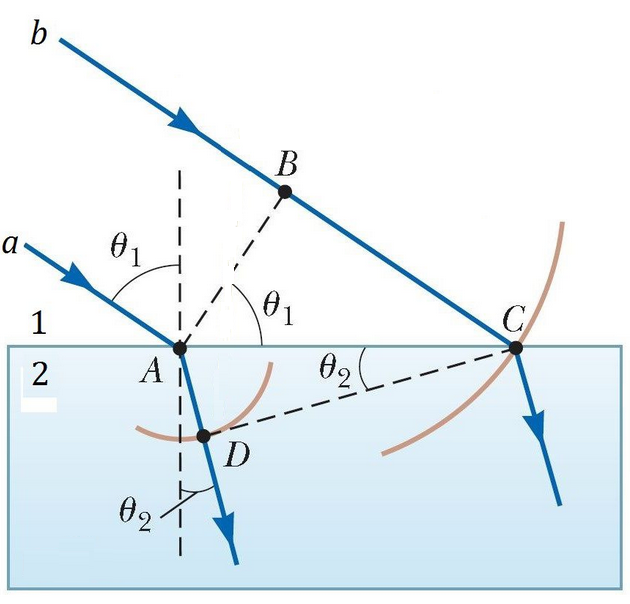
\includegraphics[width=0.55\textwidth]{4.png}
	\caption{the refraction of light}
%	\caption{the refraction of light}
\end{figure}

There are two kinds of reflection: specular and diffuse.\\

1. Specular reflection: parallel light rays are reflected from the interface and then shot out in a certain direction, and the reflected light rays can only be received in a certain direction (the reflecting surface is a smooth plane).
2. Diffuse reflection: parallel light is reflected from the interface in different directions, that is, reflected light can be received in different directions (the reflective surface is a rough plane or a curved surface).
But both specular reflection and diffuse reflection follow the law of light reflection; Diffuse reflection is an irregular reflection caused by uneven surface. It means that there are some arcs or sharp lines on the uneven surface. Suppose a ray of light hits the surface and makes its tangent line as the reflection ray.
Note: light path is reversible in light reflection.
\\

\begin{figure}
	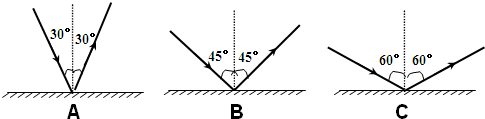
\includegraphics[width=0.75\textwidth]{5.png}
		\caption{the reflection of light}
\end{figure}
Due to the refraction and total reflection of the air, there will be a "mirage" in the air. When the sea is calm, standing on the beach, we can sometimes see high-rise buildings, streets and mountains overlapping in the distance. \cite{cJ. Geisler} There is a reason for this. When the atmosphere is relatively calm, with the increase of temperature, then the density of the air decreases too. The air temperature on the sea surface is lower than that in the air, and the refractive index of the air in the lower layer is higher than that in the upper layer. We can roughly divide the atmosphere in the air into many horizontal air layers, as shown in the lower layer which has a higher refractive index. When the light from a distant scene shoots into the air, it is constantly refracted, and the incident Angle of the upper layer with a lower refractive index becomes larger and larger. When the incident Angle of the light reaches a critical Angle, the phenomenon of total reflection will occur. The light will be high in the air through the air refraction gradually return to the next higher refractive index layer. An observer near the ground can observe an image created by light from the air, which is a mirage. When light propagates to the interface of two kinds of media, reflection and refraction usually take place at the same time. 
%\begin{figure}
%	\includegraphics[width=0.75\textwidth]{6.png}
%	%	\caption{}
%\end{figure}

%	Section	5
\section{The optical fiber}
\label{sec:Sec5}
If certain conditions are met, the light will no longer be refracted, but will all return to the original media, which is called total reflection. Total reflection is a special phenomenon of refraction of light. It can only occur when the incident Angle is greater than or equal to the critical Angle and the light shoots from the optically dense medium to the optically sparsely medium. Before the occurrence of total reflection, with the increase of the incident Angle, both the refractive Angle and the reflected Angle increase, but the refractive Angle increases rapidly. Under the condition that the intensity of the incident light is certain, the refracted light becomes weaker and weaker, and the reflected light becomes stronger and stronger. When the full emission occurs, the refracted light disappears, and the intensity of the reflected light is the same as the intensity of the incident light. That's why fiber optics are used today.
\\

It has been found that light travels along a stream of fine wine ejected from the barrel. It was also found that light can travel along curved glass rods. Since the density of medium such as water is greater than that of surrounding substances (such as air), that is, light shoots from water to air. On the surface, the light seems to bend in water. People made a transparency later which is very high, like a spider silk degree of glass -- glass fiber, when the light is at a right Angle into the glass fiber, light along the winding glass fiber. It is called an optical fiber because it can be used to transmit light.
\\

As we can see, optical fiber is usually used for some very long-distance information transmission because the loss of electricity in the wire is much higher than that of light in optical fiber. The terms fiber and cable are often confused. Most optical fibers are always hidden by some layers of protective structures which can protect them from being harmed. The covered cables are called fiber optic cables. The cover layer of the fiber can protect the fiber from the damage of the surroundings. The superfine fiber is wrapped in a plastic sheath, can be bent without fracture. The fiber is composed of two layers of different refractive index of glass composition. The inner layer is the inner core of light, with a diameter of several microns to dozens of microns, and the outer layer has a diameter of 0.1 -- 0.2mm. The refractive index of the inner glass is 0.01 higher than that of the outer glass. According to the principle of total reflection and refraction of light, when the critical angle light to the inner core and the outer interface angle is greater than the total reflection when the light does not penetrate the interface reflection. In the light of different substances in spreading at different rates, it is between the material interface are refraction and reflection. In addition, the refracted light angle as the angle of incident light change. When the incident angle reaches or exceeds a certain angle, the light will be refracted disappear, all incident light will be reflected back, this is a light reflection. Different substances refract light of the same wavelength at different angles (that is, different substances have different refractive index), and the same substance refracts light of different wavelength at different angles. Is based on the principle of optical fiber communication. Incident light is not transmitted entirely by optical fibers to the end of the optical fibers, but only in a certain angle range can the incident light be transmitted. This is called the angle of fiber numerical aperture. Large numerical aperture of optical fibers is beneficial to fiber docking. The numerical aperture of optical fibers produced by different manufacturers is different.\cite{Optical Fibre}
\\
\begin{figure}[h]
	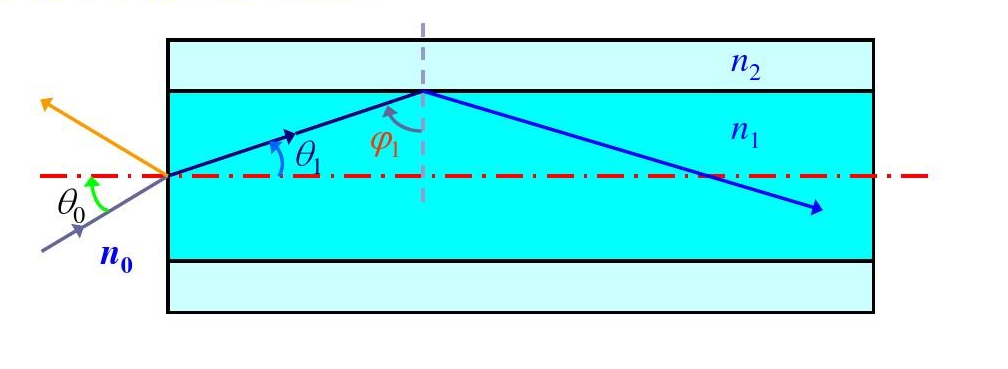
\includegraphics[width=0.75\textwidth]{7.png}
		\caption{What is optical fibre}
\end{figure}

%	Section	6
\section{Principle of optical fiber transmission}
\label{sec:Sec6}
Definition of optical fiber communication: the communication mode that takes light is the one who takes information with it as transmission medium. To understand how fiber-optic cables work, imagine an infinite length of  straw or a tube. From the start, you make up a long tube in your head. Then we assume the inner wall of it is covered by full reflector. Then, suppose you look through the pipes. From the other side, a few kilometers away, one of your friends light a match to shine it into the tube. Because that inside tube is a total reflector, the light from the flashlight will be reflected back and forth across the tube (even though the tube may be twisted), and as a result, you will see light at the other end. If your friend turns his flashlight on and off in Morse code, he can communicate with you through the channel. This is the basic principle of fiber optic cable.
\\

It is possible to make a cable from the pipe that covers the inside of the reflector, but this cable can be very thick and it is difficult to cover the inside of the pipe with a full reflector. So real fiber optic cables are made of glass. And the glass is so pure for which it is very long, but you can see the light still then. Glass is drawn into very fine strands that are as thick as a human hair. Then, cover the bread with two layers of plastic over the glass.
\\

By wrapping the glass in plastic, a mirror is created around the glass. This reflector produces a total internal reflection, just like a total reflector covered inside a tube. You can experience this reflection in a dark room with a flashlight and Windows. If you shine a flashlight at the window at an Angle of 90 degrees, the light will pass directly to the other side of the tube. But when someone aims the light at a very small Angle, the straw glass is to be a mirror. You can notice that the light reflected from the window onto the wall of the house. It is in this small angle inside the fiber transmission light is reflected, thus completely preserved inside a fiber. Telephone calls can travel via optical fibre cables, people convert the analog voice signal to digital voice signal.\cite{Optical Fibre}
\\
\begin{figure}[h]
	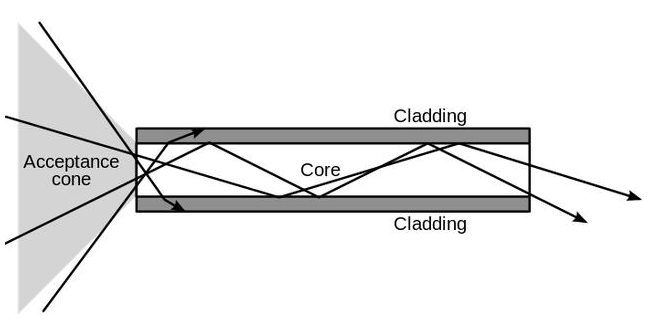
\includegraphics[width=0.75\textwidth]{9.png}
		\caption{Principle of optical fiber transmission}
\end{figure}

%	Section	7
\section{Functions of optical fiber}
\label{sec:Sec7}
There are many types of fiber, depending on the purpose, the required function and performance also vary.
\\

1. The refractive index distribution of silica fiber core and cladding is controlled by doping amount. Quartz series optical fibers have been widely used in cable TV and communication systems due to their low power consumption and wide bandwidth characteristics. Quartz glass fiber has the advantage of low loss. When the wavelength is 1.0-1.7 m, the loss is only 1 dB/km, and the lowest is 0.2 dB/km when the wavelength is 1.55 m.\cite{Optical Fibre}
\\

2. The operating wavelengths of the quartz series of optical fibers developed for optical communications are limited to 2 m, although they are used for shorter transmission distances. Therefore, it can work in the field of longer infrared wavelength. The infrared fiber is named as developed fiber. And the infrared fiber is usually applied for light energy transmission.\cite{Optical Fibre}
\\

3. Composite fiber is a kind of multi-component glass fiber made by properly mixing oxides.The characteristic of multi-component glass is that the softening point of multi-component glass is lower than that of quartz glass and the refractive index of core and cladding is very varied. And this kind of fiber is usually applied in the iatrical of optical fiber endoscopy.\cite{Optical Fibre}
\\

4. Plastic Clad Fiber USES high-purity silica glass as the core, while plastics such as silica gel with slightly lower refractive index than quartz as the cladding step type Fiber. Compared with quartz fiber, it has the characteristics of coarse core and high numerical aperture. Therefore, easy to combine with LED light source, the loss is small.\cite{Analogue optical fibre communications}
\\

5. This is an optical fiber with plastic core and cladding.It's rare but truly exists. Early products were mainly used for decoration and illumination as well as near-light optical communication. The main raw materials are plexiglass, polystyrene and polycarbonate. The loss is restricted by the inherent c-h binding structure of plastics, which can reach dozens of dB per km in general. In order to reduce the loss is developing the application fluoresso series plastics. With a core diameter of 1000 m, plastic fiber is 100 times bigger than the single one, easy to connect. As we can see, along with the progress of broadband, the development of multimode plastic fiber as a graded refractive index has been paid attention to by the society. Recently, it is applied quickly in the automobile internal LAN, and it may be applied in the family LAN in the future.\cite{Optical Fibre}
\\

6.Hollow fiber is the formation of cylindrical space, optical fiber for the transmission of light. The hollow fiber is always applied to transport energy.\cite{Optical Fibre}
\\
\begin{figure}[h]
	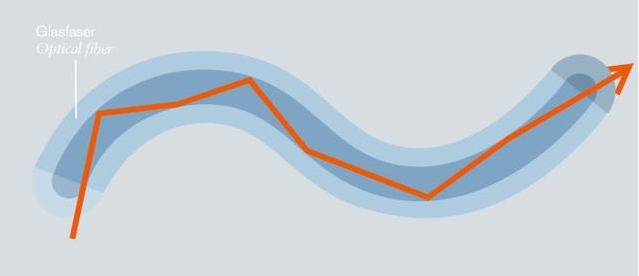
\includegraphics[width=0.65\textwidth]{8.png}
		\caption{Function of optical fibre}
\end{figure}



%	Section	8
\section{loss of optical fiber transmission}
\label{sec:Sec8}
In July 1966, Dr. Charles kao and Dr. Hockham, British Chinese of the British standard telecommunications research institute, pointed out according to the dielectric waveguide theory that the the fiber loss is not inherent and high,due to impurities in fiber.In order to realize optical fiber communication, it is important to reduce the loss of optical fiber as much as possible. \cite{Optical Fibre}
\\

There are four kinds of loss in optical fiber, namely absorption loss, scattering loss, irregular loss and bending loss.
\\

A. Optical fiber absorption loss is caused by the absorption of light energy by optical fiber materials and impurities. They consume light energy in optical fiber in the form of heat energy, which is an important loss in optical fiber. 1. Material intrinsic absorption loss, which is caused by the intrinsic absorption of material. It has two bands, one in the near infrared region of 8 to 12 m, where the band's intrinsic absorption is due to vibration. The natural absorption band of another substance in the ultraviolet band, when the absorption is strong, its tail will be dragged to 0.7 to 1.1 m band. 2. Impurity absorption, mainly optical fiber materials containing iron, copper, chromium plasma. The higher the metal ion content, the greater the loss, as long as the strict control of the metal ion content. 3. Atomic defect absorption refers to the loss caused by atomic defects in the manufacturing process of optical fiber when glass is subjected to thermal excitation or strong radiation.\cite{Analogue optical fibre communications}
\\

B. The scattering loss of optical fiber is caused by the coupling or leakage of optical power out of the fiber core due to the micro-fluctuation of atomic density in the fiber material component or the structural defect of fiber waveguide. It is due to the inhomogeneity of the atoms or molecules of the material and the structure of the material. The refractive index of the material produces microscopic inhomogeneity which results in the scattering of transmitted light waves. This scattering is inherent in the material and can not be eliminated. Rayleigh scattering is inversely proportional to the fourth power of the wavelength, and the loss caused by it can be calculated with the formula underneath:\\
$\alpha _{SR}\approx \dfrac{A}{\lambda _{0}^{4}}\left ( 1+B\Delta _{0} \right )$\cite{cJ. Geisler}\\
Where A and B are constants related to quartz and reference materials.
\\

C. Structural irregularity loss is the part of loss caused by tiny structural fluctuations at the core cladding interface and uneven waveguide structure inside the fiber. When the structure of the fiber is irregular, the mode transformation will take place, and some of the transmitted energy will be shot out of the fiber core and become radiation mode, so that the loss will be increased. This loss can be reduced by improving manufacturing techniques.
\\

D. Bending loss is the loss caused by the bending of optical fiber axis. Any deviation of the optical fiber axis visible to the naked eye from a straight line is called bending or macro bending. Fiber bending will cause the coupling between the modes in the fiber. When the energy of the propagation mode is coupled into the radiation mode or leakage mode, the bending loss will be generated. The loss increases exponentially as the radius of curvature decreases.
In the practical application of optical fiber, bending is inevitable. In order to maintain the same phase at different points on the isofacial plane, the phase velocity of optical wave needs to satisfy the following equation:\\
$\dfrac{V_{px}}{V_{pl}}=\dfrac{R+x}{R}$\cite{cJ. Geisler}\\
In the formula, R is the bending radius of the fiber, x is the distance from any point outside the fiber core to the fiber axis, and V is the phase velocity between x point and the fiber axis.\\
$x=\dfrac{(V_{px}-V_{pl})R}{V_{pl}}$\cite{cJ. Geisler}
\\


%	Section	9
\section{Image fiber transmission test}
\label{sec:Sec9}
Video signal transmission volume is growing, especially cable television, the need to send dozens of TV signals to thousands of households.In this experiment, I will adopt the method of direct modulation of analog signal to carry out the fiber transmission of video signal. The system mainly observes the fiber transmission of video signal and tests the performance of the fiber transmission analog signal. The experiment is essentially an experiment of transmitting analog signals by optical fiber.
\\

The experimental principle is as follows: the small camera generates video signal (analog signal), which is sent to the optical transmitter through analog modulation. After the fiber transmission, the optical receiver detects the video signal and outputs it to the television receiver. Then test the optical fiber transmission video signal effect and characteristics to understand the optical fiber transmission characteristics of television signals. The better the image effect, the better the performance of optical fiber transmission. Before the transmission of video signal by optical fiber, the sine wave simulation transmission is adjusted to make the peak value of sine wave and the peak value of sine wave of waveform generator the same, indicating that the waveform can be transmitted normally, which is the best transmission effect of video signal.
\\

The experimental procedure is as follows:\\
1. Connect the camera video output end with the luminous video module input end T131, and then connect T111 with a wire. The video input end of the TV set is connected with the output end T133 of the optical reception module video, and then T34 is connected to T21.\\
2. Mount 850nm optical transmitter HFBR-1414t and optical receiver HFBR-2416t, connect 1310nmT and 1310nmR with st-st fiber jumper, and form 850nm optical transmission system.\\
3. Turn the dial code switch BMI to the simulated state, and adjust the driving current of the optical generator with W112 to make the current less than 30mA.\\\cite{Analogue optical fibre communications}
4. Connect the dc power supply of the light emitting module (K10), the camera power supply and the TV power supply.\\
5. Adjust the potentiometer W111, W112 and W121 to achieve the best fiber video transmission effect.
\begin{figure}[h]
	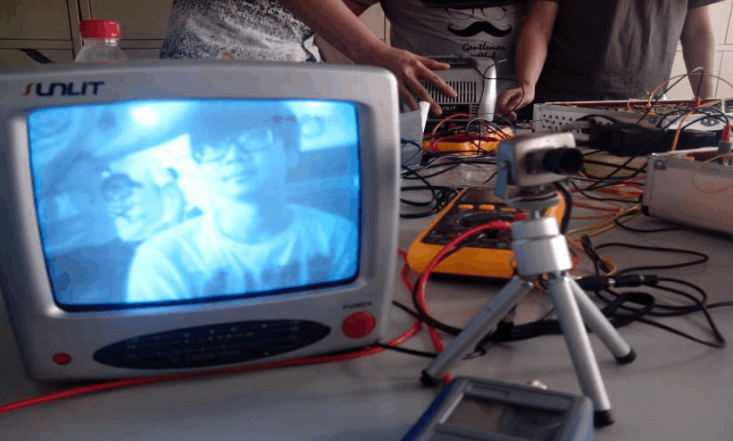
\includegraphics[width=0.55\textwidth]{11.png}
	\caption{The fiber transmission test}
%	\caption{the refraction of light}
\end{figure}

\section{Conclusions}
\label{conclusions}
We can see that in the experiment, the image effect is clear, the sensitivity is high, and it is not disturbed by electromagnetic noise. So optical fiber transmission image performance is better, and our optical fiber is small, light, long life, low price. If communication is like a road, then the wider the frequency band of the communication line, the more information it is allowed to transmit, and the larger the information capacity. Optical fiber has many applications in many fields, such as communication, computer LAN, and power system monitoring. With the progress of the society and the increasing demand for information, the transmission capacity of digital system is constantly increasing, and people urgently need to establish a unified worldwide communication network. In this situation, many shortcomings of the existing PDH are gradually exposed, mainly in North America, Western Europe and Asia, the three digital systems are not compatible with each other, there is no unified standard optical interface in the world, making the establishment of international telecommunications network and operation, management and maintenance are very complex and difficult. Millions of kilometres of fiber-optic cables have been produced since the mid-1970s, when fiber-optic communications became a reality. Ships like the global sentinel built a glass highway around the world. So far, the ships have laid some 6.44 million kilometers of fiber under the ocean floor, enough to cross the Atlantic ocean a thousand times. In addition, the continents laid 483 million kilometers of intricate optical fiber, forming what people say is a glass communication necklace. 
\\

Today, the global fibre-optic network is not only responsible for the increasing volume of network traffic, but also for the transmission of information for the world's business and banking industry, as well as connecting the world's telephone. If a Chinese had called a friend living in London more than a decade ago, the call would have been transmitted via satellite. Today, the call can be converted into a laser pulse sent over an optical fiber by simply reaching the nearest telephone system relay station. Many countries in the world are now being brought closer together by undersea cables than would have been possible even a few decades ago, let alone hundreds or thousands of years ago. Optical fiber has changed the world, the distance has died, is like this. \cite{Analogue optical fibre communications}
\\

\begin{figure}[htb]
\centering
\subfigure[pic1.]{
\begin{minipage}[t]{0.25\linewidth}
\centering
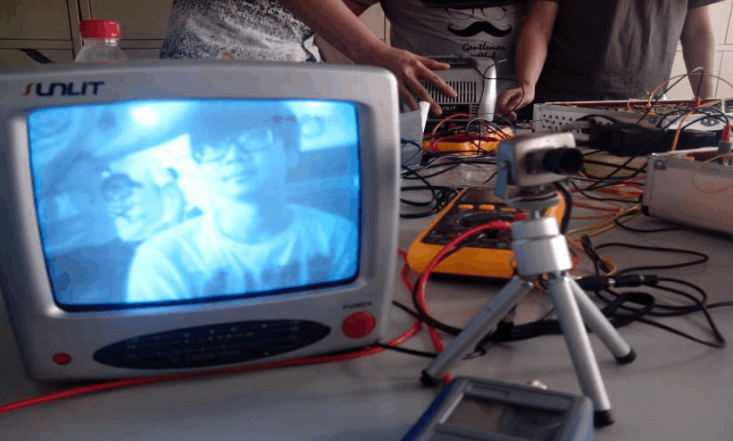
\includegraphics[width=1in]{11.png}
%\caption{fig1}
\end{minipage}%
}%
\subfigure[pic2.]{
\begin{minipage}[t]{0.25\linewidth}
\centering
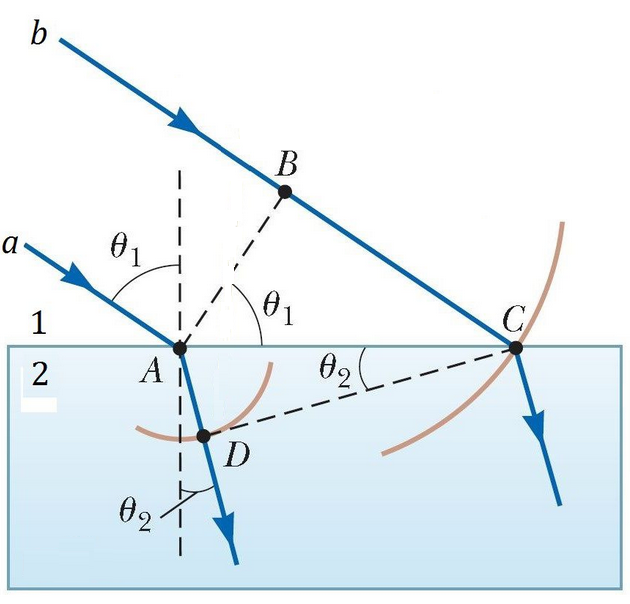
\includegraphics[width=1in]{4.png}
%\caption{fig2}
\end{minipage}%
}%
\centering
\caption{ pics}
\end{figure}
————————————————
版权声明:本文为CSDN博主「泽米」的原创文章,遵循 CC 4.0 BY-SA 版权协议,转载请附上原文出处链接及本声明。
原文链接:https://blog.csdn.net/a6822342/article/details/80533135


\vspace{6cm}
\color{black}
\noindent\rule[0.25\baselineskip]{\textwidth}{1pt}
% Bibliography
% \small
%\bibliographystyle{unsrt}




\begin{thebibliography}{10}


\bibitem{Tarja Volotinen}
Tarja Volotinen and Willem Griffioen
\newblock Reliability of optical fibres and components.
\newblock {\em Reliability of optical fibres and components}, 1999.



\bibitem{cJ. Geisler}
cJ. Geisler,Beaven and J.P.Boutruche.
\newblock 
\newblock {\em Optical fibres}, 1986.

    \bibitem{Optical Fibre}
Kao;Charles K; Institution of Eletrical Engineers.
\newblock Optical Fibre
\newblock {\em Optical Fibre}, 1998

\bibitem{Analogue optical fibre communications}
Wilson;Brett; Ghassemloooy; Zabih; Darwazeh; Izzat
\newblock Analogue optical fibre communications
\newblock {\em Analogue optical fibre communications}, 1995.


\end{thebibliography}





\end{document}